\section{Results}

\subsection{Five screens, one protocol}
Of six candidate confirmation datasets, four met the pre-specified inclusion rules (Table~\ref{tab:inclusion}). The Adamson unfolded-protein-response screen has no cell labelled \texttt{control} in the harmonised file. The Dixit screen labels conditions by guide, which leaves 27 qualifying conditions, below the minimum of 30. Both were excluded as the plan required, rather than by adjusting rules after inspection. Together with the discovery dataset, the study covers \numNPerturbationsTotal{} single-gene perturbations: \numNNorman{} in Norman (K562, CRISPRa), \numNReplogleKEssential{} and \numNReplogleRpe{} in the Replogle K562 and RPE1 CRISPRi screens, and \numNTianCrispra{} and \numNTianCrispri{} in the Tian iPSC-derived-neuron CRISPRa and CRISPRi screens. The confirmation screens come from two studies: the two Replogle screens are different cell lines profiled in one study with one platform, and the two Tian screens are activation and interference in one neuronal system. They are therefore not four independent replications.

\begin{table}[t]
\centering\small
\caption{Datasets and pre-specified inclusion outcomes. Perturbations are single-gene conditions with enough cells whose target is a measured gene. Batches are 10x lanes or the dataset's batch annotation.}
\label{tab:inclusion}
\resizebox{\linewidth}{!}{\begin{tabular}{llllrrp{4.3cm}}
\toprule
Dataset & Role & Status & Perturbations & Controls & Batches & Exclusion reason \\
\midrule
Norman K562 CRISPRa & Discovery & Included & 105 & 9,702 & 8 &  \\
Replogle K562 CRISPRi & Confirmation & Included & 1,663 & 10,691 & 48 &  \\
Replogle RPE1 CRISPRi & Confirmation & Included & 1,378 & 11,485 & 56 &  \\
Adamson K562 CRISPRi (UPR) & Confirmation & Excluded & -- & -- & -- & no cells labelled control (guide-level labels only) \\
Dixit K562 knockout (day 7) & Confirmation & Excluded & -- & 5,381 & -- & guide-level labels: 27 qualifying conditions ($<$30) \\
Tian neurons CRISPRa & Confirmation & Included & 97 & 434 & 2 &  \\
Tian neurons CRISPRi & Confirmation & Included & 183 & 437 & 4 &  \\
\bottomrule
\end{tabular}}
\end{table}

\subsection{How much of a perturbation's response is measurable varies widely across screens}
We first asked how reproducible each perturbation-specific response is, meaning the response minus the mean response of other perturbations. Each response was re-estimated from two disjoint sets of batches, each set with its own batch-matched controls. The resulting technical reproducibility limits (Spearman--Brown estimates of the correlation that a noiseless predictor could reach \emph{within the same experiment}) were \numLimNorman{} for Norman (95\% CI \numLimLoNorman--\numLimHiNorman), \numLimReplogleRpe{} for RPE1 (\numLimLoReplogleRpe--\numLimHiReplogleRpe), \numLimReplogleKEssential{} for K562 (\numLimLoReplogleKEssential--\numLimHiReplogleKEssential), \numLimTianCrispra{} for Tian CRISPRa (\numLimLoTianCrispra--\numLimHiTianCrispra) and \numLimTianCrispri{} for Tian CRISPRi (\numLimLoTianCrispri--\numLimHiTianCrispri) (Supplementary Table~\ref{tab:limits}). Four further random partitions of batches changed these by at most 0.02. Tian CRISPRa has only two batches, so every partition compares batch 1 with batch 2, and its limit rests on a single batch contrast. Splitting cells at random instead of by batch gave similar values, except in Tian CRISPRa (\numLimCellsTianCrispra), where the batch contrast lowers the estimate. These limits describe technical reproducibility (sampling and lane-to-lane variation within one experiment). They omit biological replicate variation, so they are upper bounds for prediction within these experiments, not for predicting an independently repeated experiment. The specific response reproduced ($r\ge0.5$) for \numFracReproNorman\% of Norman perturbations, \numFracReproReplogleRpe\% (RPE1), \numFracReproReplogleKEssential\% (K562), \numFracReproTianCrispra\% (Tian CRISPRa) and \numFracReproTianCrispri\% (Tian CRISPRi).

Measurement reliability in turn limits how well any metric can \emph{discriminate} informative from uninformative predictions (Fig.~\ref{fig:calibration}; Supplementary Table~\ref{tab:discrimination}). A technical duplicate beat the mean of other perturbations on MSE for \numWinMeanNormanMse{} of Norman perturbations (95\% Wilson CI \numWinMeanLoNormanMse--\numWinMeanHiNormanMse), \numWinMeanReplogleRpeMse{} in RPE1, \numWinMeanReplogleKEssentialMse{} in K562, and \numWinMeanTianCrispraMse{} and \numWinMeanTianCrispriMse{} in the neuron screens. This reflects the data rather than a defect of the metric. MSE is a proper scoring rule, and its win rate tracks reproducibility closely: within K562, the duplicate won on MSE for \numMseWinLowReplogleKEssential{} of the least reproducible third of perturbations and \numMseWinHighReplogleKEssential{} of the most reproducible third (RPE1: \numMseWinLowReplogleRpe{} and \numMseWinHighReplogleRpe; Supplementary Table~\ref{tab:discrel}). Where a perturbation's specific response is below the noise, no metric can separate a correct prediction from an uninformative one. Perturbation-specific correlation always ranks a duplicate above the mean, because the mean has no defined specific correlation. Against a zero prediction (post hoc), however, the duplicate won for \numWinZeroNormanPearsonSpecific{} of Norman perturbations, \numWinZeroReplogleRpePearsonSpecific{} in RPE1 and \numWinZeroReplogleKEssentialPearsonSpecific{} in K562, and for almost none in the neuron screens. The planned threshold of 80\% for an adequate metric was met for MSE only in Norman. We treat the win rate as continuous and draw conclusions from several metrics and from aggregates over perturbations.

\begin{figure}[t]
\centering
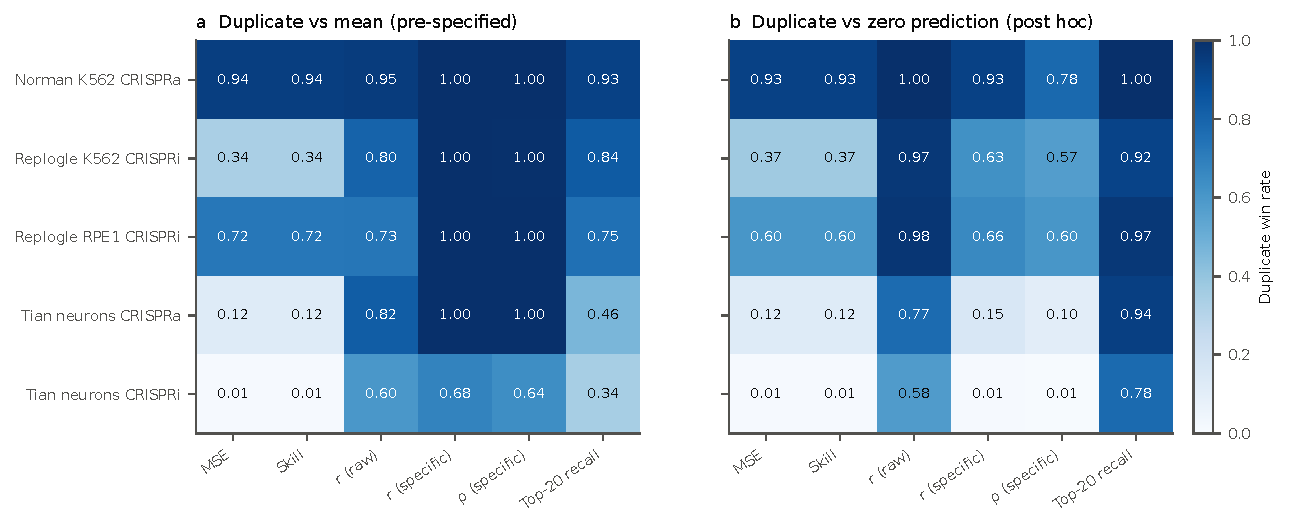
\includegraphics[width=\linewidth]{figures/fig6_calibration.pdf}
\caption{\textbf{Metric discrimination.} Fraction of single-gene perturbations for which a technical duplicate (the response from half of the cells and controls) scores better than an uninformative prediction of the other half. \textbf{a}, against the mean of other perturbations (pre-specified, addendum E4). \textbf{b}, against a zero prediction (post hoc). The two comparisons are separate; the better baseline is never chosen per perturbation. Undefined correlations of uninformative predictions count as 0. Wilson intervals are in Supplementary Table~\ref{tab:discrimination}.}
\label{fig:calibration}
\end{figure}

\subsection{Unseen genes: small but reproducible gains in large screens only}
The pre-specified confirmatory test C1 asked whether any learned model had lower MSE than the mean of training perturbations on held-out genes (Table~\ref{tab:c1}). The prediction of the discovery analysis, that none would, was \emph{refuted} in both Replogle screens: ridge regression, gene-loading ridge and the MLP ensemble all had lower MSE than the mean (all Holm-adjusted $p<0.001$; \numNCOneBeat{} of \numNCOneTests{} tests). The gains were small. Skill relative to the mean was \numSkillReplogleKEssentialMlpEnsemble{} (95\% CI \numSkillLoReplogleKEssentialMlpEnsemble--\numSkillHiReplogleKEssentialMlpEnsemble) for the MLP in K562 and \numSkillReplogleRpeMlpEnsemble{} (\numSkillLoReplogleRpeMlpEnsemble--\numSkillHiReplogleRpeMlpEnsemble) in RPE1, so the models removed about 5\% of the squared error left by the mean (Fig.~\ref{fig:unseen}a). The result was stable across three alternative fold partitions (Supplement). In the discovery dataset, no model was better than the mean (MLP skill \numSkillNormanMlpEnsemble, CI \numSkillLoNormanMlpEnsemble{} to \numSkillHiNormanMlpEnsemble). Norman is the screen where metrics discriminate best, so this is a genuine negative result rather than a measurement artefact.

In the neuron screens, no model met the pre-specified criterion, but one came close and the result needs care. In Tian CRISPRa, the MLP's signed-rank test was significant after Holm correction ($p_{\mathrm{Holm}}=0.0098$), but the bootstrap interval of its mean MSE difference included zero (Table~\ref{tab:c1}). The two parts of the rule disagree because the per-perturbation differences are skewed (Supplementary Fig.~\ref{fig:c1dist}). The MLP was better for \numTianAMlpFracBetter\% of perturbations, with a median difference of \numTianAMlpMedian{} ($\times10^{-3}$; 95\% CI \numTianAMlpMedianLo{} to \numTianAMlpMedianHi), but a few large losses brought the mean difference to \numTianAMlpMean. We therefore report that the MLP was typically, but not on average, better than the mean in this screen. The effect is small (skill \numSkillTianCrispraMlpEnsemble), in a screen where MSE has almost no power to discriminate, so we give it little weight in either direction. Beyond that, the C1 result in the neuron screens is uninformative rather than negative. With about 430 control cells, the training mean carries control-sampling noise that disjoint evaluation controls correctly fail to reward: predicting no change scored skill \numZeroSkillTianCrispra{} and \numZeroSkillTianCrispri{} relative to the mean.

Perturbation-specific correlations followed the same pattern (Fig.~\ref{fig:unseen}b). They reached \numSpecReplogleKEssentialMlpEnsemble{} (K562) and \numSpecReplogleRpeMlpEnsemble{} (RPE1) for the MLP, far below the technical reproducibility limits of \numCeilBatchReplogleKEssential{} and \numCeilBatchReplogleRpe. They were also only modestly above two controls: an MLP with permuted co-expression features (\numShufSpecReplogleKEssentialMlpEnsemble, \numShufSpecReplogleRpeMlpEnsemble), and the zero prediction (\numZeroSpecReplogleKEssential, \numZeroSpecReplogleRpe). Gains concentrated in perturbations whose responses are reproducible (post hoc). To avoid selecting on the outcome being scored, we selected perturbations using two cell halves within one set of batches, and scored the models against the response estimated from the other set, which shares no perturbed cells or batch-matched control cells with the selection. In K562, among the \numRiNReplogleKEssentialRidgeRep{} perturbations reproducible in the selection set, ridge reached skill \numRiSkillReplogleKEssentialRidgeRep{} (95\% CI \numRiLoReplogleKEssentialRidgeRep--\numRiHiReplogleKEssentialRidgeRep) and the MLP \numRiSkillReplogleKEssentialMlpEnsembleRep{} (\numRiLoReplogleKEssentialMlpEnsembleRep--\numRiHiReplogleKEssentialMlpEnsembleRep), against \numRiSkillReplogleKEssentialRidgeAll{} and \numRiSkillReplogleKEssentialMlpEnsembleAll{} over all perturbations scored the same way. In RPE1 (\numRiNReplogleRpeMlpEnsembleRep{} perturbations), the MLP reached \numRiSkillReplogleRpeMlpEnsembleRep{} (\numRiLoReplogleRpeMlpEnsembleRep--\numRiHiReplogleRpeMlpEnsembleRep). In Norman, nothing improved on the mean even among its \numRiNNormanRidgeRep{} reproducible perturbations (ridge \numRiSkillNormanRidgeRep, MLP \numRiSkillNormanMlpEnsembleRep). The neuron screens had too few reproducible perturbations (\numRiNTianCrispraRidgeRep{} and \numRiNTianCrispriRidgeRep) to assess.

\paragraph{Robustness (post hoc).} The Replogle results held under each sensitivity analysis (Supplementary Tables~\ref{tab:genesets}--\ref{tab:cellcount}):
\begin{itemize}
\item \emph{Output genes.} Scoring all detected genes rather than the 2{,}000 selected genes and targets gave MLP skill \numGsReplogleKEssentialMlpEnsembleExtended{} (K562) and \numGsReplogleRpeMlpEnsembleExtended{} (RPE1), and \numGsReplogleKEssentialMlpEnsembleOutsidePrimary{} and \numGsReplogleRpeMlpEnsembleOutsidePrimary{} on the genes outside the selected set. The harmonised Replogle files contain only genes expressed in the screen, so genes induced from silence can only be scored in Norman and the neuron screens, where no model beat the mean on them either.
\item \emph{Control-cell splits.} MLP skill ranged from \numCsMinReplogleKEssentialMlpEnsemble{} to \numCsMaxReplogleKEssentialMlpEnsemble{} (K562) and from \numCsMinReplogleRpeMlpEnsemble{} to \numCsMaxReplogleRpeMlpEnsemble{} (RPE1) across five independent control splits.
\item \emph{Initialisation.} MLP skill ranged from \numSeedMinReplogleKEssentialMlpEnsemble{} to \numSeedMaxReplogleKEssentialMlpEnsemble{} and from \numSeedMinReplogleRpeMlpEnsemble{} to \numSeedMaxReplogleRpeMlpEnsemble{} across five seeds.
\item \emph{Dependence between perturbations.} Targets share pathways and programmes, so we also resampled clusters of co-expressed targets rather than single perturbations (block bootstrap). Intervals for the primary C1 estimand, mean $\Delta$MSE, still excluded zero for all six Replogle tests. On mean skill, the MLP's intervals stayed above zero (K562 \numBlockLoReplogleKEssentialMlpEnsemble--\numBlockHiReplogleKEssentialMlpEnsemble; RPE1 \numBlockLoReplogleRpeMlpEnsemble--\numBlockHiReplogleRpeMlpEnsemble), but those of the linear models widened to include zero in RPE1 (ridge \numBlockLoReplogleRpeRidge--\numBlockHiReplogleRpeRidge).
\item \emph{Cell counts.} Skill was higher for perturbations measured in more cells (MLP in K562: \numCcFewestReplogleKEssentialMlpEnsemble{} in the third with fewest cells, \numCcMostReplogleKEssentialMlpEnsemble{} in the third with most), and excluding conditions with fewer than 100 cells raised it to \numCcHundredReplogleKEssentialMlpEnsemble{} (RPE1: \numCcHundredReplogleRpeMlpEnsemble).
\end{itemize}

\begin{table}[t]
\centering\scriptsize
\caption{Confirmatory test C1: learned models versus the mean baseline on held-out genes. $\Delta$MSE is the mean per-perturbation difference (model $-$ mean), multiplied by $10^3$; negative favours the model. $p$: one-sided Wilcoxon signed-rank; Holm correction across all 12 tests. ``Beats mean'' requires $p_{\mathrm{Holm}}<0.05$ and a 95\% bootstrap interval below 0.}
\label{tab:c1}
\resizebox{\linewidth}{!}{\begin{tabular}{llcrrrc}
\toprule
Dataset & Model & $\Delta$MSE$\times10^{3}$ vs mean (95\% CI) & Skill & $p$ & $p_{\mathrm{Holm}}$ & Beats mean \\
\midrule
Replogle K562 CRISPRi & Ridge & -0.231 (-0.280, -0.187) & 0.025 & $<$0.001 & $<$0.001 & yes \\
Replogle K562 CRISPRi & Gene-loading ridge & -0.214 (-0.267, -0.165) & 0.018 & $<$0.001 & $<$0.001 & yes \\
Replogle K562 CRISPRi & MLP ensemble & -0.274 (-0.331, -0.220) & 0.051 & $<$0.001 & $<$0.001 & yes \\
Replogle RPE1 CRISPRi & Ridge & -0.428 (-0.572, -0.296) & 0.011 & $<$0.001 & $<$0.001 & yes \\
Replogle RPE1 CRISPRi & Gene-loading ridge & -0.380 (-0.519, -0.251) & 0.010 & $<$0.001 & $<$0.001 & yes \\
Replogle RPE1 CRISPRi & MLP ensemble & -0.480 (-0.646, -0.324) & 0.052 & $<$0.001 & $<$0.001 & yes \\
Tian neurons CRISPRa & Ridge & +0.023 (+0.007, +0.043) & -0.010 & 0.99 & 1 & no \\
Tian neurons CRISPRa & Gene-loading ridge & +0.005 (+0.000, +0.011) & -0.001 & 0.96 & 1 & no \\
Tian neurons CRISPRa & MLP ensemble & -0.008 (-0.036, +0.023) & 0.012 & 0.0016 & 0.0098 & no \\
Tian neurons CRISPRi & Ridge & +0.000 (-0.000, +0.001) & -0.000 & 0.96 & 1 & no \\
Tian neurons CRISPRi & Gene-loading ridge & +0.000 (-0.000, +0.000) & -0.000 & 0.23 & 1 & no \\
Tian neurons CRISPRi & MLP ensemble & +0.001 (-0.001, +0.002) & -0.001 & 0.91 & 1 & no \\
\bottomrule
\end{tabular}}
\end{table}

\begin{figure}[t]
\centering
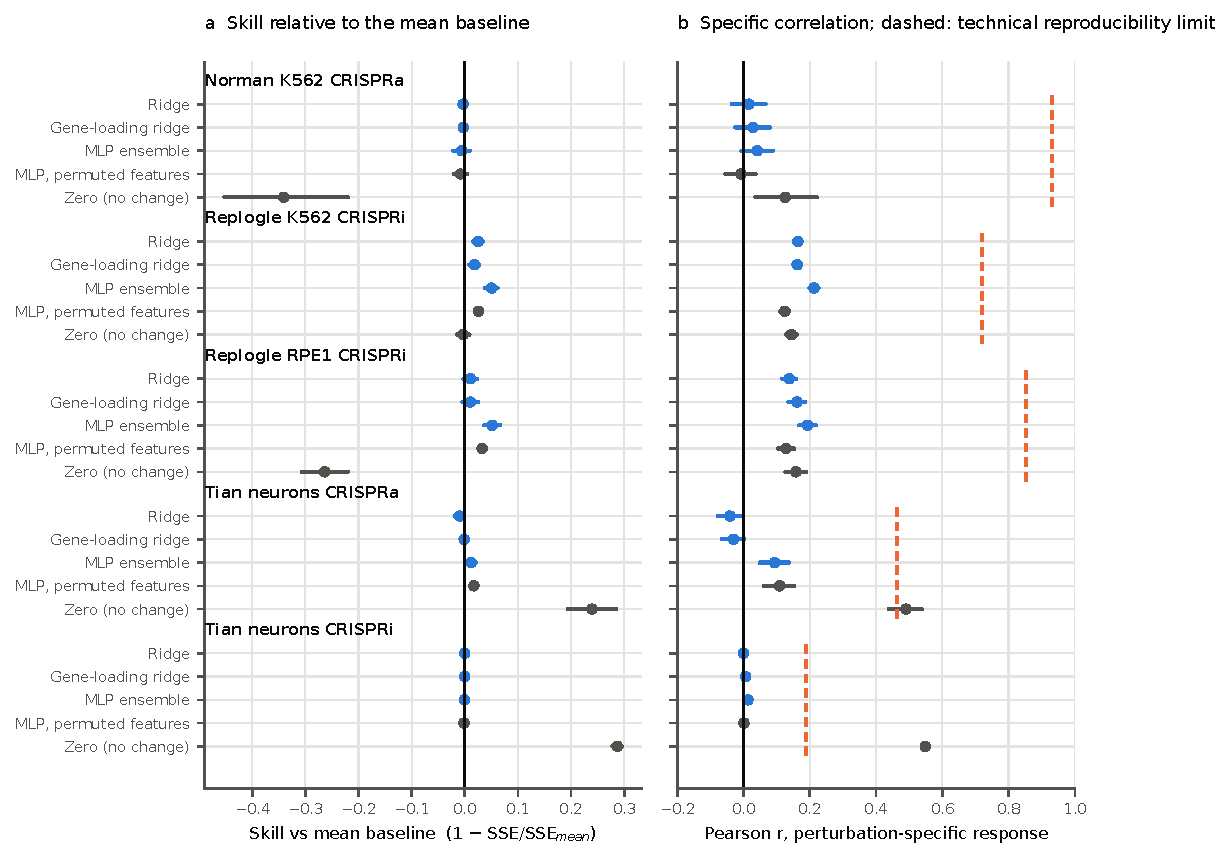
\includegraphics[width=\linewidth]{figures/fig2_unseen_genes.pdf}
\caption{\textbf{Prediction for genes absent from training.} Means over held-out perturbations with 95\% bootstrap intervals (5 folds, seed 0). Blue: pre-specified learned models with co-expression features. Grey: controls, namely the MLP with co-expression features permuted among genes (target baseline expression retained) and the zero prediction. \textbf{a}, skill relative to the training mean (0 = mean baseline). \textbf{b}, Pearson correlation of the perturbation-specific response, with the batch-disjoint technical reproducibility limit (dashed).}
\label{fig:unseen}
\end{figure}

\subsection{Co-expression features help in large screens; pretrained Gene2vec does not add to them}
Test C2 compared co-expression features with the same features permuted among genes; both kept the target's own control-cell expression. Co-expression improved skill for both ridge and the MLP in both Replogle screens (\numNCTwoInformative{} of \numNCTwoTests{} tests), but not in the neuron screens (Table~\ref{tab:c2c3}). The plan specified no multiplicity correction for C2. With a post-hoc Holm correction over its eight two-sided Wilcoxon tests, all four Replogle results remain significant (largest adjusted $p=\numCTwoMaxHolmReplogle$) and none of the neuron results are ($p_{\mathrm{Holm}}\ge\numCTwoMinHolmTian$). This shows that co-expression carries information about an unseen gene's response. It does not show that the information is practically useful: the gains are a few hundredths of skill (Table~\ref{tab:c2c3}). Test C3 asked whether frozen Gene2vec embeddings, trained on co-expression across 984 public datasets \citep{du2019gene2vec}, improve on co-expression from the screen's own control cells. They did not in general. Gene2vec was significantly \emph{worse} for ridge in K562. Only one of \numNCThreeTests{} tests favoured Gene2vec (MLP, Tian CRISPRi), by a skill difference of about 0.002, which is of no practical consequence. For the MLP in K562, the Holm-adjusted signed-rank test was significant ($p<0.001$) while the bootstrap interval of the mean skill difference included zero (\numCThreeMeanReplogleKEssentialMlpEnsemble). The cause is the same as in C1: the median difference was \numCThreeMedianReplogleKEssentialMlpEnsemble{} (95\% CI \numCThreeMedianLoReplogleKEssentialMlpEnsemble{} to \numCThreeMedianHiReplogleKEssentialMlpEnsemble), and Gene2vec was better for only \numCThreeFracReplogleKEssentialMlpEnsemble\% of perturbations. Gene2vec was thus typically slightly worse, but the average difference is uncertain. Mean and median estimates for every confirmatory test are in Supplementary Table~\ref{tab:estimands}.

\begin{table}[t]
\centering\scriptsize
\caption{Confirmatory tests C2 and C3 on held-out genes. Skill differences are per-perturbation paired means with 95\% bootstrap intervals. C2 is supported (co-expression informative) if the interval lies above 0. C3 uses a two-sided Wilcoxon test, Holm-corrected across its 8 tests.}
\label{tab:c2c3}
\resizebox{\linewidth}{!}{\begin{tabular}{lllllcc}
\toprule
Test & Contrast & Dataset & Model & Skill difference (95\% CI) & $p_{\mathrm{Holm}}$ & Supported \\
\midrule
C2 & Co-expression $-$ permuted & Replogle K562 CRISPRi & Ridge & +0.028 (+0.019, +0.035) & -- & yes \\
C2 & Co-expression $-$ permuted & Replogle K562 CRISPRi & MLP ensemble & +0.025 (+0.013, +0.035) & -- & yes \\
C2 & Co-expression $-$ permuted & Replogle RPE1 CRISPRi & Ridge & +0.018 (+0.005, +0.030) & -- & yes \\
C2 & Co-expression $-$ permuted & Replogle RPE1 CRISPRi & MLP ensemble & +0.019 (+0.005, +0.033) & -- & yes \\
C2 & Co-expression $-$ permuted & Tian neurons CRISPRa & Ridge & -0.009 (-0.017, -0.002) & -- & no \\
C2 & Co-expression $-$ permuted & Tian neurons CRISPRa & MLP ensemble & -0.005 (-0.010, +0.000) & -- & no \\
C2 & Co-expression $-$ permuted & Tian neurons CRISPRi & Ridge & +0.000 (-0.000, +0.001) & -- & no \\
C2 & Co-expression $-$ permuted & Tian neurons CRISPRi & MLP ensemble & +0.001 (-0.000, +0.002) & -- & no \\
C3 & Gene2vec $-$ co-expression & Replogle K562 CRISPRi & Ridge & -0.029 (-0.038, -0.019) & $<$0.001 & no \\
C3 & Gene2vec $-$ co-expression & Replogle K562 CRISPRi & MLP ensemble & -0.008 (-0.017, +0.004) & $<$0.001 & no \\
C3 & Gene2vec $-$ co-expression & Replogle RPE1 CRISPRi & Ridge & -0.008 (-0.023, +0.005) & 1 & no \\
C3 & Gene2vec $-$ co-expression & Replogle RPE1 CRISPRi & MLP ensemble & -0.004 (-0.017, +0.010) & 1 & no \\
C3 & Gene2vec $-$ co-expression & Tian neurons CRISPRa & Ridge & +0.008 (+0.001, +0.018) & 0.78 & no \\
C3 & Gene2vec $-$ co-expression & Tian neurons CRISPRa & MLP ensemble & -0.002 (-0.009, +0.006) & 1 & no \\
C3 & Gene2vec $-$ co-expression & Tian neurons CRISPRi & Ridge & +0.000 (-0.000, +0.000) & 1 & no \\
C3 & Gene2vec $-$ co-expression & Tian neurons CRISPRi & MLP ensemble & +0.002 (+0.000, +0.003) & 0.029 & yes \\
\bottomrule
\end{tabular}}
\end{table}

\subsection{What co-expression features carry (post hoc)}
To separate the components of the primary features, we refit ridge and the MLP on the primary folds with each component alone (Fig.~\ref{fig:ablation}; Supplementary Table~\ref{tab:ablation}). In both Replogle screens, co-expression alone matched the full feature set: MLP skill \numAblReplogleKEssentialMlpEnsembleCoexpressionOnly{} versus \numAblReplogleKEssentialMlpEnsembleFull{} in K562, and \numAblReplogleRpeMlpEnsembleCoexpressionOnly{} versus \numAblReplogleRpeMlpEnsembleFull{} in RPE1. The target's own control-cell expression level and detection rate behaved differently for the two models. With these two baseline features alone, the MLP reached about two-thirds of the full gain (\numAblReplogleKEssentialMlpEnsembleBaselineBoth{} and \numAblReplogleRpeMlpEnsembleBaselineBoth), whereas ridge reached almost none (\numAblReplogleKEssentialRidgeBaselineBoth{} and \numAblReplogleRpeRidgeBaselineBoth).

A large part of the usable signal is therefore available from how strongly and how broadly the target is expressed in unperturbed cells. The relation is not a simple monotonic one: target expression correlates only weakly with response magnitude (Spearman $\rho=0.16$ in K562 and $0.06$ in RPE1, post hoc), so the MLP's gain from these two features reflects nonlinear structure that our analyses do not resolve. The co-expression embedding largely subsumes this signal (adding the baseline features changed skill by at most 0.005) and adds a further component that a linear model can use. That component is consistent with broad transcriptional programmes shared by co-regulated genes, rather than with mechanism-specific information. These features are statistical associations measured in unperturbed cells, and our analyses do not show that they reflect causal regulatory relationships.

Because the control-derived features had used control cells from both random halves, including the half behind the evaluation targets, we recomputed them from the training half alone. Performance was unchanged: MLP skill \numAblReplogleKEssentialMlpEnsembleFullSplit{} (K562) and \numAblReplogleRpeMlpEnsembleFullSplit{} (RPE1), against \numAblReplogleKEssentialMlpEnsembleFull{} and \numAblReplogleRpeMlpEnsembleFull{} with the primary features. The results do not depend on that overlap.

\begin{figure}[t]
\centering
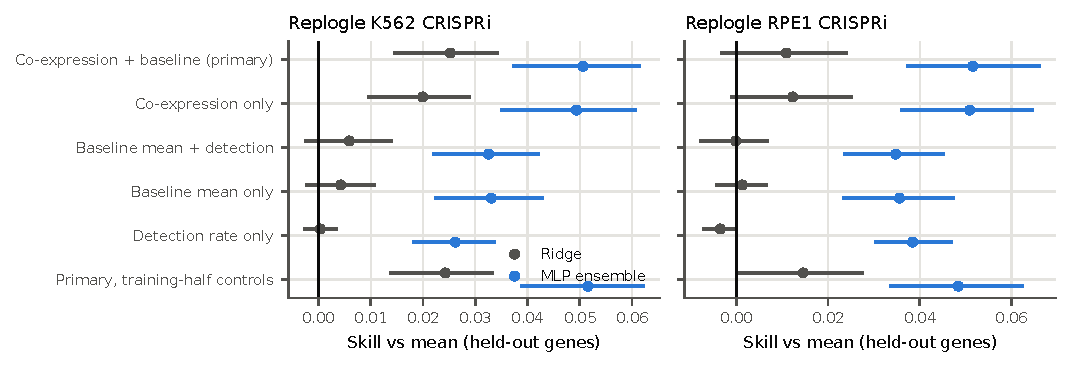
\includegraphics[width=0.95\linewidth]{figures/fig7_feature_ablation.pdf}
\caption{\textbf{Feature ablation in the large screens} (post hoc). Skill on held-out single genes with each feature component alone, and with the primary features recomputed from training-half control cells only. Means with 95\% bootstrap intervals; grey: ridge, blue: MLP ensemble.}
\label{fig:ablation}
\end{figure}

\subsection{Within a screen, gains grow with the number of training perturbations}
Subsampling training perturbations within fixed folds of the two Replogle screens (exploratory E1) showed a steady increase without a clear plateau (Fig.~\ref{fig:size}). Specific correlation rose from about 0.04 with 25 training perturbations to \numLcSpecFullReplogleKEssentialRidge{} (K562) and \numLcSpecFullReplogleRpeRidge{} (RPE1) with all of them, about 1{,}000, roughly linearly in the logarithm of training size. Skill rose too but remained small (ridge: \numLcFullReplogleKEssentialRidge{} and \numLcFullReplogleRpeRidge{}). With around 70 training perturbations, the size of the Norman training folds, skill in the Replogle screens is near zero and specific correlation below 0.1, consistent with the failure in the discovery screen. This is an association within one study's screens, from three draws per size. Screens also differ in modality, cell type, depth and number of controls, so the curves do not establish that training-set size is the main determinant of performance across experiments.

\begin{figure}[t]
\centering
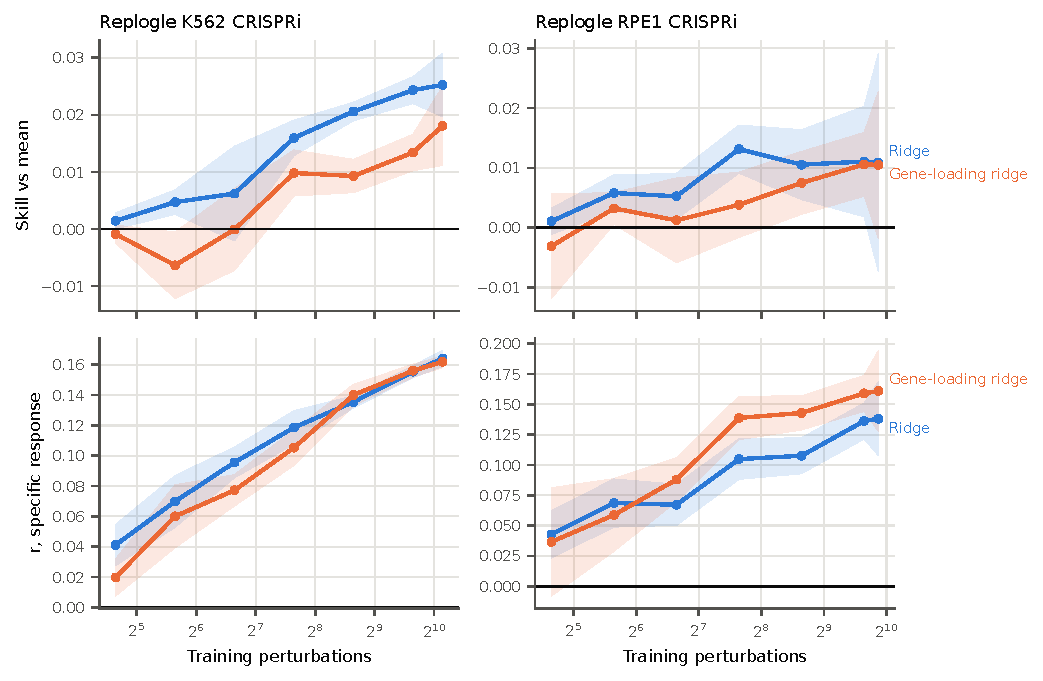
\includegraphics[width=0.92\linewidth]{figures/fig3_training_size.pdf}
\caption{\textbf{Performance against training-set size} (exploratory). Training perturbations subsampled within each fold (three draws per size), with test perturbations fixed. Means over folds and draws $\pm$1.96 standard errors.}
\label{fig:size}
\end{figure}

\subsection{A measurement in another cell line is about as informative as the best model}
For \numNSharedKToRpe{} genes knocked down in both Replogle screens (exploratory E2), the measured response in one cell line was a poor predictor in the other when used as is (skill \numCcTransferRawKToRpe{} for K562$\to$RPE1, \numCcTransferRawRpeToK{} for RPE1$\to$K562), because responses differ systematically in scale between the lines (Fig.~\ref{fig:cross}). Taking the source screen's specific response, rescaled by one factor fitted on other genes and added to the target screen's mean, gave skill \numCcTransferDeviationScaledKToRpe{} (\numCcLoTransferDeviationScaledKToRpe--\numCcHiTransferDeviationScaledKToRpe) and \numCcTransferDeviationScaledRpeToK{} (\numCcLoTransferDeviationScaledRpeToK--\numCcHiTransferDeviationScaledRpeToK), with specific correlation \numCcSpecTransferDeviationScaledKToRpe{} in both directions. That is comparable to the best unseen-gene model on the same targets. In this one pair of cell lines, a direct measurement of the same perturbation in the other line therefore carried about as much transferable gene-specific information as the models extract within the target screen. The two predictors use different information, a measurement elsewhere versus learned structure, and one rescaling factor is a simple transfer model, so this comparison is exploratory and may not hold for other pairs of contexts or modalities.

\begin{figure}[t]
\centering
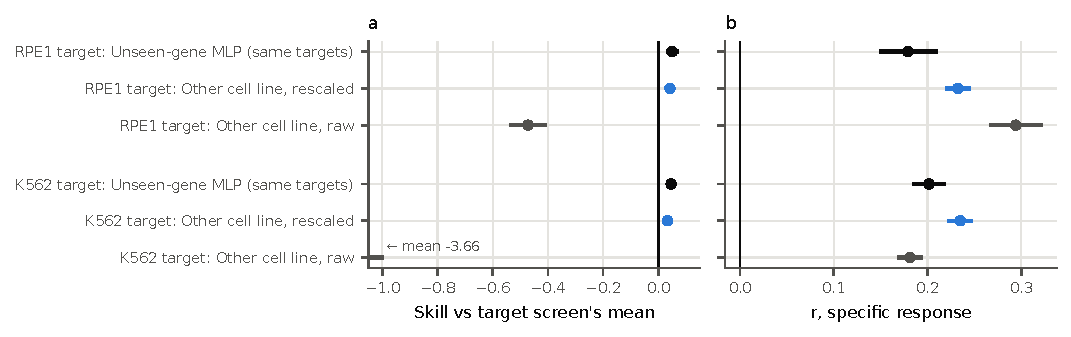
\includegraphics[width=0.95\linewidth]{figures/fig4_cross_context.pdf}
\caption{\textbf{Transfer between cell lines} (exploratory). Targets knocked down in both Replogle screens, scored on genes measured in both. ``Rescaled'': the target screen's mean plus the source screen's specific response, multiplied by one factor fitted on other targets. The unseen-gene MLP is shown on the same targets, scored on the target screen's full gene set.}
\label{fig:cross}
\end{figure}

\subsection{Ranking strong responders}
For prioritising experiments, the relevant question is whether the strongest responses can be found among untested genes (Supplementary Table~\ref{tab:ranking}). In K562, the top 20\% of held-out genes by predicted response magnitude contained \numRkReplogleKEssentialRidgeTwenty{} (ridge; 95\% CI \numRkLoReplogleKEssentialRidgeTwenty--\numRkHiReplogleKEssentialRidgeTwenty) of the truly strongest 20\%, against 0.20 expected by chance. In RPE1 the figure was \numRkReplogleRpeRidgeTwenty{} (\numRkLoReplogleRpeRidgeTwenty--\numRkHiReplogleRpeRidgeTwenty). Both were significant against random rankings at the 10\%, 20\% and 30\% thresholds (permutation $p<0.01$), and stable across MLP seeds (\numRkSeedMinReplogleKEssential--\numRkSeedMaxReplogleKEssential{} and \numRkSeedMinReplogleRpe--\numRkSeedMaxReplogleRpe{} at 20\%). In Norman and the neuron screens, rankings were not distinguishable from random. An enrichment of 1.5- to 3-fold, depending on screen and threshold, is statistically clear, but we have not shown that it would change experimental decisions; that requires prospective validation.

\subsection{Selected gene pairs: attenuated additive projection, captured by a single scale factor}
In the discovery screen, pairs whose single-gene responses were measured were predicted well by the sum of the singles (skill \numPairskillAdditive{} relative to the mean of pairs). A single global scale factor applied to that sum, fitted on training pairs, raised skill to \numPairskillScaledAdditive. Ridge and MLP models of the residual from the additive prediction reached \numPairskillRidgeOnAdditive{} and \numPairskillMlpOnAdditive, but their MSE was not distinguishable from the scaled sum (difference \numPairMseDiffScaled, 95\% CI \numPairMseDiffScaledLo{} to \numPairMseDiffScaledHi; Fig.~\ref{fig:pairs}b).

Because noise in the estimated single responses would bias a fitted scale factor towards zero, we estimated it per pair with an instrumental-variable estimator using independent halves of the single-perturbation cells. The median coefficient was \numBetaIvMedian{} (95\% CI \numBetaIvLo--\numBetaIvHi; least squares \numBetaOlsMedian), and \numFracBelowOne\% of the \numNPairs{} pairs were below 1 (Fig.~\ref{fig:pairs}a). The single responses were measured reliably (median split-half $r$ \numSinglesReliability), so the correction was small. For most of these pairs, the response projects less strongly onto the sum of the single responses than additivity would predict. A coefficient below 1 does not by itself establish biological sub-additivity. It is also consistent with weaker knockdown or activation by guides in the double-perturbation construct, with response components orthogonal to the additive direction, or with differences in cell state, survival or capture between single- and double-perturbation conditions. Moreover, the instrumental-variable correction assumes that the two halves of the single-gene cells measure the same response with independent errors. The pairs were chosen from a genetic-interaction map \citep{norman2019} and are enriched for interactions, and no other included screen contains pairs. We therefore report an attenuated additive projection among selected, interaction-enriched pairs, not a general property of combined perturbations.

\begin{figure}[t]
\centering
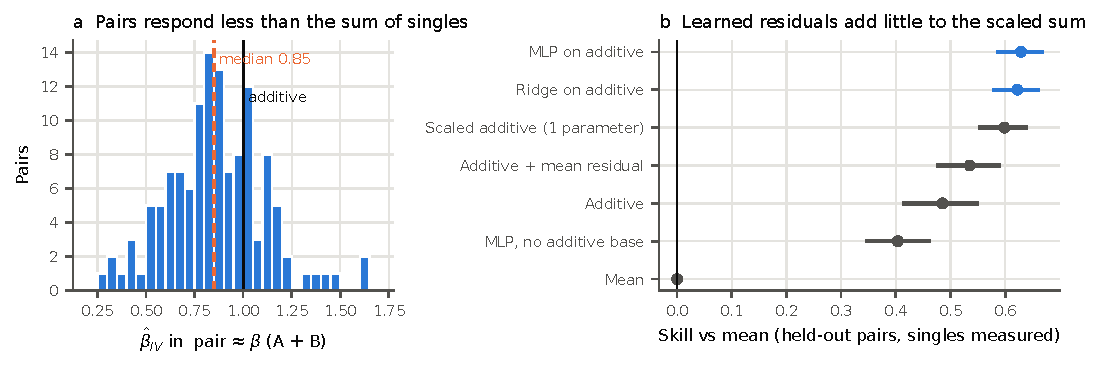
\includegraphics[width=\linewidth]{figures/fig5_pairs.pdf}
\caption{\textbf{Gene pairs in the discovery screen} (exploratory). \textbf{a}, per-pair coefficient $\beta$ in pair $\approx\beta\,$(A+B), estimated with an instrumental variable to remove attenuation from measurement error. \textbf{b}, skill on held-out pairs whose singles were measured; models in blue learn a residual from the additive prediction.}
\label{fig:pairs}
\end{figure}

\subsection{Prediction intervals}
Per-gene 90\% intervals calibrated on held-out residuals covered \numCovReplogleKEssential{} (K562), \numCovReplogleRpe{} (RPE1) and \numCovNorman{} (Norman) of genes overall. On each perturbation's 20 genes with the largest \emph{predicted} deviation from the mean, which is how genes would be chosen in practice, coverage was close to nominal: \numIvPredReplogleKEssentialMlpEnsemble{}, \numIvPredReplogleRpeMlpEnsemble{} and \numIvPredNormanMlpEnsemble{} for the MLP (Supplementary Table~\ref{tab:ivsel}). On the 20 genes with the largest \emph{observed} deviation, coverage fell to \numCovTopReplogleKEssential, \numCovTopReplogleRpe{} and \numCovTopNorman. That subset is selected on the outcome and preferentially contains large errors, so its low coverage does not show that the intervals are miscalibrated. It does show a practical limitation: the genes that turn out to respond most strongly are largely not the ones the models predict, so intervals are wide enough on average but rarely contain the extreme responses. Calibrating within strata of predicted magnitude did not change this (Supplementary Table~\ref{tab:intervals}).
